\documentclass[conference]{IEEEtran}
\IEEEoverridecommandlockouts
% The preceding line is only needed to identify funding in the first footnote. If that is unneeded, please comment it out.
\usepackage{cite}
\usepackage{amsmath,amssymb,amsfonts}
\usepackage{algorithmic}
\usepackage{graphicx}
\usepackage{textcomp}
\usepackage{hyperref}
\usepackage{xcolor}
\def\BibTeX{{\rm B\kern-.05em{\sc i\kern-.025em b}\kern-.08em
    T\kern-.1667em\lower.7ex\hbox{E}\kern-.125emX}}
\begin{document}

\title{Humanoid Sprinting and Stopping DRL}

\author{

    \IEEEauthorblockN{Carlos Veríssimo}
    \IEEEauthorblockA{\textit{Department of Informatics Engineering} \\
        \textit{FEUP}\\
        Porto, Portugal \\
        up201907716@up.pt }
    \and

    \IEEEauthorblockN{Miguel Amorim}
    \IEEEauthorblockA{\textit{Department of Informatics Engineering } \\
        \textit{FEUP}\\
        Porto, Portugal \\
        up201907756@up.pt }
    \and

    \IEEEauthorblockN{Rafael Camelo}
    \IEEEauthorblockA{\textit{Department of Informatics Engineering } \\
        \textit{FEUP}\\
        Porto, Portugal \\
        up201907729@up.pt }
}


\maketitle

\begin{abstract}

This paper thoroughly examines the challenges of sprinting in the RoboCup 3D Simulation League, employing a simulated NAO robot. Our goal is to enhance the understanding of these complexities, paving the way for the development of optimized soccer-playing robots. Specifically, we concentrate on refining humanoid robot running, drawing inspiration from FC Portugal's advancements using Proximal Policy Optimization (PPO) reinforcement learning. The study reviews related works, details our methodology, and discusses key results. Emphasizing the importance of Team Description Papers (TDP) for league participation, our work aligns with the innovative spirit of RoboCup, offering insights into future directions in robotics and AI.

\end{abstract}

\begin{IEEEkeywords}
    RoboCup, RoboCup 3D Simulation League, Reinforcement Learning, Humanoid Sprinting, Humanoid Stopping, Soccer
\end{IEEEkeywords}

\section{Introduction}

Reinforcement learning (RL) is a machine learning field in which agents learn optimal behaviours through trial-and-error interactions with their environment to maximize rewards and minimize punishments.

The RoboCup, which began in 1997, is a well-known platform for promoting robots and AI by pushing participants with tasks such as soccer, rescue, and home care. \cite{robocup97}.

This article digs into RoboCup's 3D Simulation League, introduced in 2004. The league evolved from using simple spheres to humanoid robots and now uses a simulated version of the NAO robot, a 58-cm-tall robot with 25 degrees of freedom (DOF) \cite{naorobot}, as the robot model.

\begin{figure}[htbp]
    \centerline{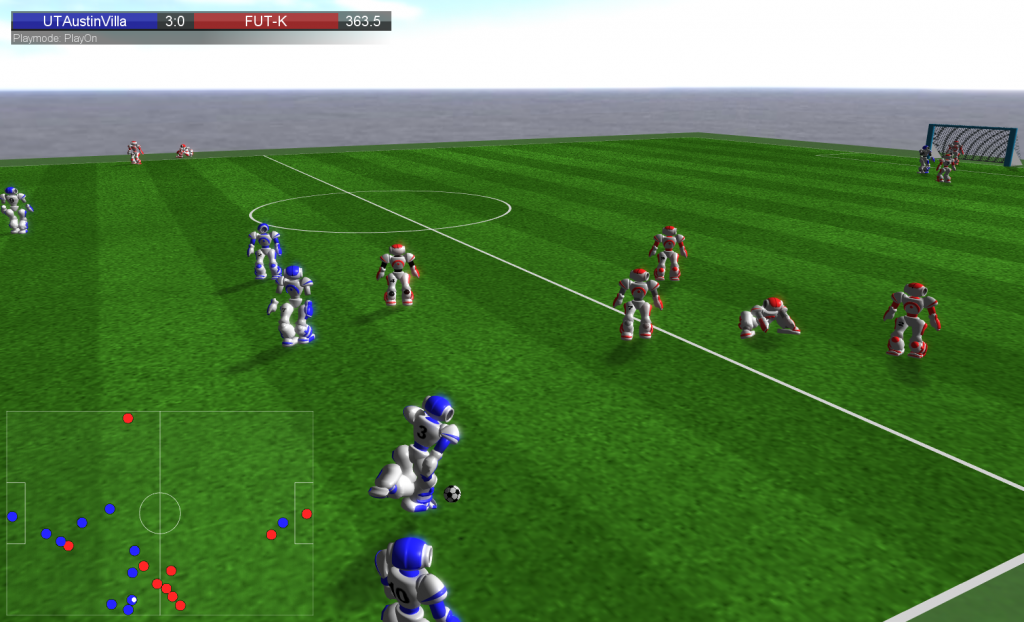
\includegraphics[width=0.35\textwidth]{images/robocup3d.png}}
    \caption{RoboCup 3D Simulation League.}
    \label{fig:robocup3d}
\end{figure}

To enforce physics laws, coordinate communications between the server and clients, and officiate the game, the league uses the SimSpark simulator.

Sprinting is an important feature of robotic soccer and plays a key role in team success. This paper also focuses on the difficult problem of stopping a run without falling, a feat that necessitates detailed control over the robot's numerous joints and sensors.

This study focuses on improving humanoid robot running and halting in the RoboCup 3D Simulation League.
Recognizing the intricacy and significance of these talents in robotic soccer, we intend to expand on previous advances in the field.
Our primary goal is to create solid, reliable techniques for accelerating and decelerating without falling by making use of comprehensive control
of the robot's joints and sensors.

We intend to build upon FC Portugal's efforts to improve humanoid robot running and stopping, and will use existing Gym environments to train our agent.
The FC Portugal's team repository can be found \href{https://github.com/m-abr/FCPCodebase}{https://github.com/m-abr/FCPCodebase}

This repository was created to ease the development of a team for the RoboCup 3D Simulation League.
It contains a set of tools and scripts that allow the user to train and test a team of simulated robots.

Subsequent sections detail related works (Section \ref{Related Work}), our methodology (Section \ref{Methodology}),
the significant results and their implications (Section \ref{Results and Discussion}),
concluding with future directions for this field (Section \ref{Conclusions and Future Work})

\section{Related Work}\label{Related Work}

The RoboCup is an annual event that showcases new techniques and algorithms in robotics and AI research. One of its leagues, the 3D Simulated Soccer League, has become particularly noteworthy for its contribution to the field. Participating teams are required to submit a Team Description Paper (TDP) outlining their prior research and development initiatives.

Recently, FC Portugal submitted a TDP \cite{lau2020fc} that introduced two new skills in humanoid sprinting and stopping, which were learned through a Proximal Policy Optimization (PPO) reinforcement learning algorithm. The team utilized all joints but the head to control the robot's movement, with angles controlled using a proportional controller.

The sprinting skill is focused on running in a straight line, with the skill ending in one of three ways: the robot kicks the ball, transitions to walking, or stops. The running skill yields the same outcomes as sprinting, except that the robot does not kick the ball. Abreu et al. \cite{10.1007/978-3-030-35699-6_1} describes the team's efforts to leverage the PPO algorithm using the simulator's information to learn how to run faster, more stably, and stop.

The team implemented the PPO algorithm provided by OpenAI's Baselines library, which used clipped surrogate objectives and alternated between data sampling and stochastic gradient ascent. The authors adapted hyperparameters from OpenAI's work with a 3D humanoid model in mujoco, making adjustments for their specific tasks.

The experimental setup and testing were the same as the sprinting behavior, with the robot placed near the left goal and facing the other goal. The objective was to run as quickly as possible in a straight line, with rewards based on the torso's x-coordinate difference from the last step. After stabilizing the sprinting behavior at around 2.5 m/s, the team trained the stopping behavior only after optimizing the running behavior. The robot was placed in the same initial pose as before and ran for some time until the stopping behavior was triggered.

\section{Methodology}\label{Methodology}

In this section, we outline the key components of our simulator and the agent used for training and testing.
The primary objective is to design an environment for training a humanoid agent that can both sprint and stop without falling.

The functionality is encapsulated in a Python script:

\textbf{Reset function} to initialize and stabilize the robot's state at the beginning of each training episode.
The robot is initially positioned above ground level, with its posture aligned using an existing behavior, 'Zero\textunderscore Bent\textunderscore Knees'. Subsequently, it is beamed to the ground.
This function is crucial for ensuring a consistent starting state, allowing for accurate assessment of the robot's learning progress.


\textbf{Step function}, responsible for executing the actions derived from the reinforcement learning algorithm.
It modifies the robot's step behavior and joint positions based on the input actions, fostering exploration and varied movement patterns. The function also monitors for terminal conditions, such as falls or timeouts, crucial for defining the boundaries of each training episode.

\subsection{Simulator and Agent}\label{Simulator and Agent}

As mentioned before, we intend to use FC Portugal's team repository as a basis for our work.

An integration with OpenAI gym is provided, which allows us to use the gym environment to train, test and evaluate our agent.

Simspark is used as the simulator, which is a 3D simulator for humanoid robots. It serves as the underlying physics engine that replicates the physical world in which our agent operates.
It allows us to model sprinting and stopping behaviours realistically, providing a high-fidelity simulation environment.

The agent used is a simulated representation of the NAO robot.

\subsection{State Space}\label{State Space}

The state space represents the information available to the agent at each time step. It includes various sensory inputs and internal variables that capture the robot's state within the SimSpark environment.
Our state space is composed of 70 variables, describing the robot's position, orientation, velocities, accelerations, and angles of all joints.

Figure \ref{fig:nao-joints} shows the robot's joints.

\begin{figure}[htbp]
    \centerline{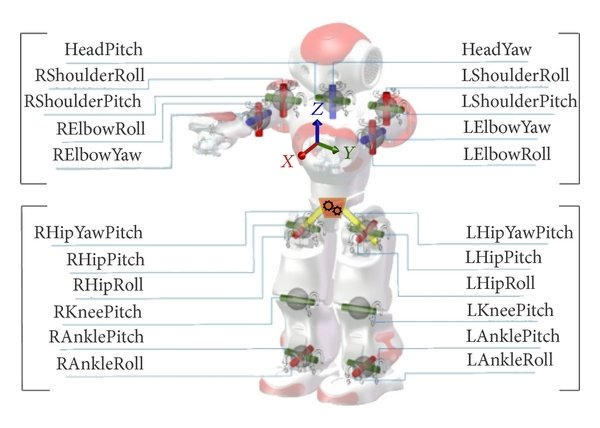
\includegraphics[width=0.35\textwidth]{images/joints.png}}
    \caption{Nao's joints.}
    \label{fig:nao-joints}
\end{figure}

\subsection{Action Space}\label{Action Space}

The action space defines the set of actions that the agent can take to interact with the SimSpark environment. Our action space comprises 22 continuous dimensions, each of which corresponds to a specific joint or motion parameter. These actions allow the agent to control its movements and execute complex motor actions within the simulator.

\subsection{Reward Function}\label{Reward Function}

The reward function is structured to assess various aspects of the robot's walking behaviour, each contributing to a cumulative score that reflects the efficacy and naturalness of its movements.

The reward function is composed of 7 components, each with a different weight, which are summed to obtain the final reward:
\begin{itemize}
    \item \textbf{Arm Coordination and Movement}: The function evaluates the coordination between the robot's arms, rewarding movements where the arms swing in opposite directions.
          reminiscent of human walking. This aspect encourages not only coordination but also ensures that arm movements contribute positively to overall balance and momentum.
    \item \textbf{Leg Coordination}: Similar to arm coordination, leg movements are rewarded based on their coordinated and alternating action. This evaluation is crucial for a bipedal gait, as it promotes a stable and efficient step cycle.
    \item \textbf{Opposite Arm and Leg Coordination}: Emulating the natural human gait, the reward function encourages the opposite movement of arms and legs. This coordination is vital for maintaining balance and forward momentum.
    \item \textbf{Posture and Elevation Penalties}: To discourage a posture that might lead to instability or falls, the robot is penalized for low torso and head heights. Maintaining an upright position is fundamental for effective bipedal locomotion.
    \item \textbf{Head Stability}: Stability in the robot's head movement is rewarded, as excessive oscillation can disrupt balance and visual processing, which are essential for navigating complex environments.
    \item \textbf{Joint Movement Reward}: Movement in the robot's joints, particularly in the limbs, contributes positively to the reward. This aspect ensures that the robot does not remain static and encourages the dynamic movement essential for walking.
    \item \textbf{Forward Movement Incentive}: One of the primary goals of the reward function is to promote forward movement. The robot earns rewards for advancing, whereas moving backwards incurs penalties. This aspect is crucial for achieving the primary objective of walking.
    \item \textbf{Torso Orientation}: An upright or slightly forward-leaning torso orientation is rewarded. This posture is typical of human walking and helps maintain balance and forward momentum.
\end{itemize}

Out of all the components mentioned above, leg and arm coordination and movement are the most important
ones, as they are the ones that most influence the robot's stability and forward movement.

\subsection{Optimization Algorithm}\label{Optimization Algorithm}

The chosen optimization algorithm is Proximal Policy Optimization (PPO), developed by OpenAI \cite{ppo-openai}

It focuses on optimizing the agent's policy, i.e., the state-action mapping, by maximizing the expected reward, \cite{ppo}.

Small updates to the policy are made at each iteration, based on the collected experience, to improve the agent's performance. These updates are constrained to avoid large policy changes.

The algorithm encourages exploration by using a stochastic policy, which allows the agent to learn from experience and discover new, potentially better, policies, balancing the exploration-exploitation trade-off.

The algorithm trains in multiple epochs, where each epoch consists of a fixed number of iterations through
the collected data.

Figure \ref{fig:training} shows the training setup for the sprinting behaviour.

\begin{figure}[htbp]
    \centerline{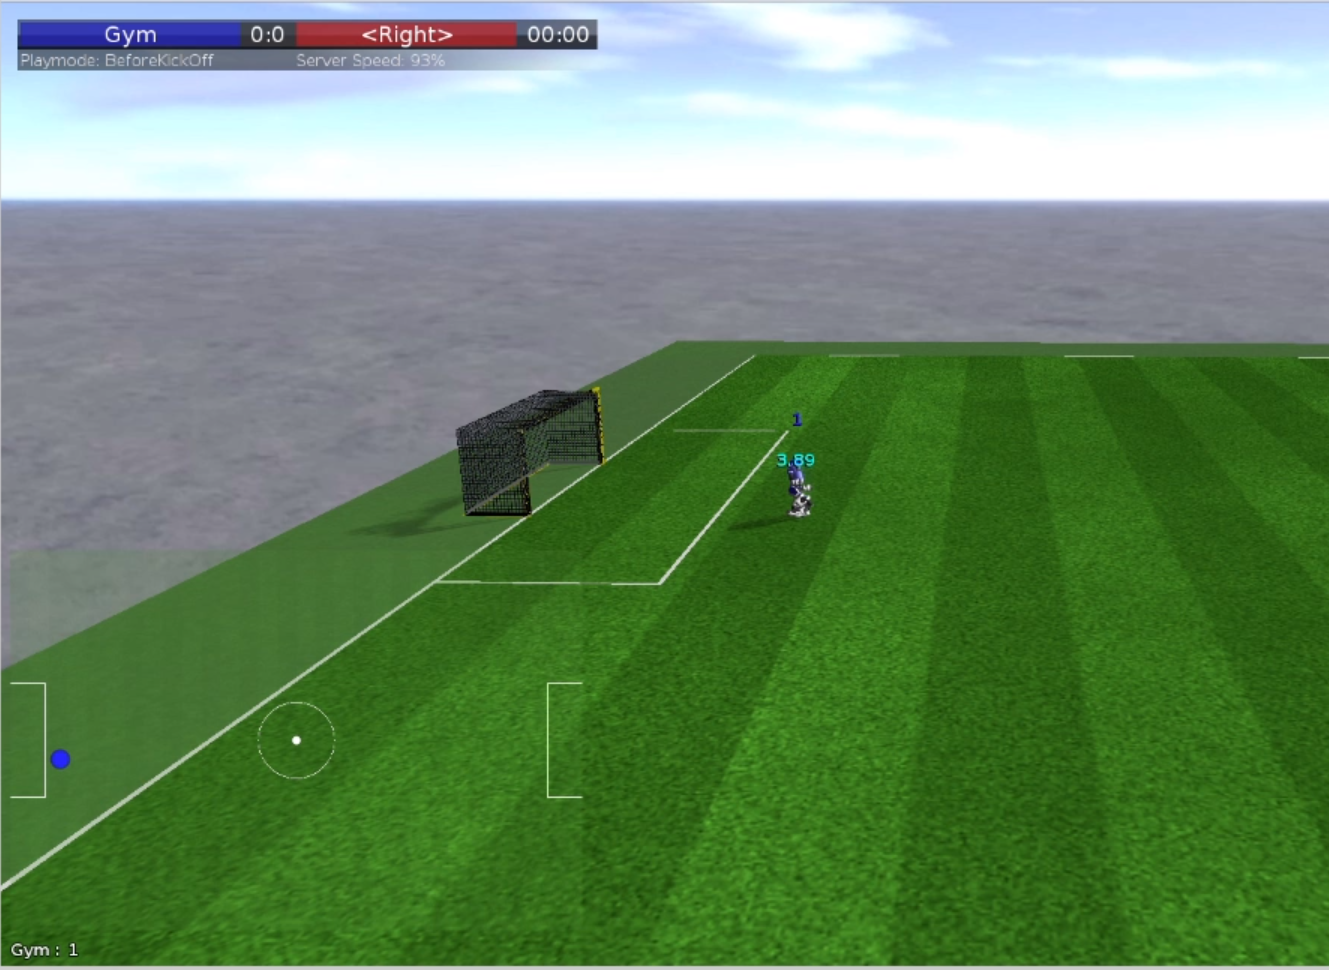
\includegraphics[width=0.4\textwidth]{images/training.png}}
    \caption{The training setup}
    \label{fig:training}
\end{figure}


\section{Results and Discussion}\label{Results and Discussion}

In the pursuit of developing this robot project, significant progress was made in enabling the robot to walk and even run. We were implementing complex coding mechanisms and intricate algorithms that allowed for dynamic and coordinated movements, showcasing the potential for mobility. However, despite these accomplishments, a noteworthy challenge emerged in the form of an inability to make the robot come to a halt.

We encountered difficulties in creating an effective reward function that would encourage the robot to perform the tasks we intended. In some cases, our reward system led to unexpected results where the robot learned that remaining stationary was the most rewarding behaviour, rather than engaging in the desired activities like walking or running

Additionally, fine-tuning the components of the reward function mentioned in \ref{Reward Function} proved challenging. Adjusting these details was crucial to guide the robot towards the intended behaviors, but finding the right balance required careful experimentation and adjustments

Our model training was conducted on a computer equipped with an Intel i7 10th generation processor. With this setup, the average duration for each training session was approximately 2 hours.

In our experiments, the best-performing model achieved an average reward of 3.63, with the maximum possible reward being 7.3. This outcome indicates that while the model has learned to some extent, there is still significant room for improvement in terms of optimizing the reward function and enhancing the model's overall performance


The stumbling block primarily stemmed from persistent issues within the coding framework utilized. Various debugging attempts were made to rectify the problem, yet the solution remained elusive. This hiccup underscored the intricate nature of simultaneously achieving fluid locomotion and precise control. Moving forward, addressing and refining the underlying code will be a paramount focus to ensure seamless movement and the crucial ability to bring the robot to a complete stop. This experience highlights the iterative nature of robotics development and emphasizes the importance of meticulous coding for comprehensive functionality.

\section{Conclusions and Future Work}\label{Conclusions and Future Work}

In conclusion, our project has achieved notable milestones despite not meeting all our initial goals. We successfully trained the model to enable the NAO robot to run within the Simspark environment, though with a less human-like motion than anticipated. This accomplishment marks a significant step in our understanding and application of complex concepts in robot learning and control.

Throughout this project, we have gained extensive experience in several key areas:

\begin{itemize}
    \item \textbf{Familiarization with Simspark}: We delved deeply into this 3D simulation platform, understanding its intricacies and leveraging its capabilities for our robotic simulations.
   \item \textbf{Robot Learning Principles}: Our work contributed to a deeper understanding of the principles behind robot learning, particularly in the context of reinforcement learning and its application to robotic movements.
   \item{Controlling Robot Joints: We developed skills in manipulating and controlling the NAO robot's joints, a crucial aspect of achieving desired movement patterns.}
\end{itemize}

Although our project didn't fully realize the planned run-and-stop functionality, the progress made lays a strong foundation for future endeavours. The insights and expertise we have garnered through this process are invaluable and will undoubtedly fuel further advancements in robotic control and learning.

% FUTURE WORK SECTION
With additional time and computational resources, future work on this project could significantly enhance the capabilities of the NAO robot in the simulation. The primary focus would be on three key areas:

\begin{enumerate}
    \item \textbf{Improved Stopping Mechanism}: training the robot to stop efficiently and safely from higher speeds. This requires a complex understanding and simulation of momentum, balance, and actuator control.
    \item \textbf{Smoother Running Motion}: refining the robot's running gait to make it less jerky and more fluid. This involves intricate tuning of the robot's motor commands and real-time adjustments based on its dynamics and interaction with the environment.
    \item \textbf{Multi-Directional Running}: Expanding the robot's ability to run in various directions, not just forward. This adds an element of agility and adaptability, enabling the robot to navigate more complex environments with turns and obstacles.
\end{enumerate}

In future iterations of our project, harnessing cloud computing platforms such as Google Cloud Platform (GCP), Amazon Web Services (AWS), and Microsoft Azure could markedly improve the efficiency and scope of our training process. Cloud computing offers access to greater computational power and resources, enabling more extensive and efficient training of our robotic agent. Utilizing these platforms could significantly reduce training times and allow for more complex and computationally demanding models to be explored. This approach could lead to quicker iterations, more sophisticated learning algorithms, and potentially a more refined and capable robotic behavior



\section{Acknowledgments}\label{Acknowledgments}

First and foremost, we would like to express our gratitude for the collaboration and cooperation we have maintained throughout this relatively brief yet intricate task.

We would also like to extend our gratitude to the members involved in the development of FC Portugal's team repository for their work and for making it available to the public.

\begin{thebibliography}{00}
    \bibitem{lau2020fc}Lau, N., Reis, L., Simoes, D., Abreu, M., Silva, T. \& Resende, F. FC Portugal 3D Simulation Team: Team Description Paper 2020.  (2023)
    \bibitem{10.1007/978-3-030-35699-6_1}Abreu, M., Reis, L. \& Lau, N. Learning to Run Faster in a Humanoid Robot Soccer Environment Through Reinforcement Learning. {\em RoboCup 2019: Robot World Cup XXIII}. pp. 3-15 (2019)
    \bibitem{naorobot} Nao the Humanoid and Programmable Robot, \href{www.aldebaran.com/en/nao}{www.aldebaran.com/en/nao}. Last accessed 24 Dec 2023
    \bibitem{robocup97} Noda, I., Suzuki, S. J., Matsubara, H., Asada, M., Kitano, H.: RoboCup-97: The first robot world cup soccer games and conferences. AI magazine 19(3), 49-49 (1998)
    \bibitem{ppo} Proximal Policy Optimization (PPO) Explained, \href{https://towardsdatascience.com/proximal-policy-optimization-ppo-explained-abed1952457b}{https://towardsdatascience.com/proximal-policy-optimization-ppo-explained-abed1952457b}. Last accessed 3 Jan 2024
    \bibitem{ppo-openai} Proximal Policy Optimization, \href{https://openai.com/research/openai-baselines-ppo}{https://openai.com/research/openai-baselines-ppo}. Last accessed 3 Jan 2024
\end{thebibliography}

\end{document}
